% espacio entre parrafos
\setlength{\parskip}{5mm}
% sangria
\setlength{\parindent}{5mm}

\linespread{1.1}%
\selectfont	

\section{Introducción}

\emph{Ginga} es una especificación de un \textit{middleware} que permite la ejecución 
de aplicaciones interactivas en un receptor de TV Digital terrestre.
La especificación de \emph{Ginga} se encuentra descripta  en la 
norma ABNT NBR 15606.

% y agrega a la norma
% ISDB-Tb la posibilidad de utilizar aplicaciones interactivas.


Los receptores de TV Digital , que funcionan de acuerdo al 
Sistema Argentino de Televisión Digital Terrestre (SATVD-T), deben contar con 
una  implementación del \textit{middleware} \emph{Ginga}. 

\emph{Ginga.ar} es una implementación de dicho estándar, desarrollada por el laboratorio
LIFIA de la Universidad Nacional de La Plata, a partir de la implementación 
de referencia de Ginga-NCL creada por la PUC de Rio de Janeiro. \emph{Ginga.ar} está 
desarrollado  en C++, es Software Libre y las licencias utilizadas son GPLv2 
y LGPLv2.

\emph{Ginga.ar} permite ejecutar aplicaciones interactivas   escritas en NCL 
(\textit{Nested Context Language}). 
NCL es  un lenguaje de aplicación XML con elementos diseñados para la 
especificación de  los aspectos de la interactividad, la sincronización 
espacio-temporal de los  objetos multimedia, la adaptación y soporte 
para múltiples dispositivos.

\emph{Ginga.ar} fue portado a diversas plataformas de STB equipadas con  
\textit{chip-sets} diferentes, entre ellos ST7101, ST7102, ST7105 y ST7108 que poseen 
una
arquitectura SH4. También a \textit{chip-sets} de arquitectura ARM, como los CS1200 y 
CS1800.
\emph{Ginga.ar} además se ejecuta en distribuciones Linux \textit{desktop} de 32 y 64 bits, 
además de Windows.

Este documento presenta la arquitectura, herramientas y librerías necesarias para el desarrollo y extensión de Ginga.ar.
También se incluyen detalles sobre los principales módulos y clases que lo componen.
Finalmente, se explica, mediante diagramas de secuencia UML, cómo interactuan diferentes componentes del middleware para ciertos casos de interés.

\section{Tecnologías y herramientas de desarrollo}
Para el desarrollo de Ginga se puede utilizar un entorno de desarrollo integrado (IDE), como Eclipse-CDT o Kdevelop, así también como trabajar
desde un editor de texto y una terminal. Mínimamente se requiere de un compilador C++, preferiblemente GCC a partir de la versión 4.6.3, un interprete de python
(a partir de la versión 2.7.3), y CMake a partir de su versión 2.8. Con estas tres herramientas más las librerías externas requeridas (listadas luego),
se tiene todo lo necesario para compilar el código fuente de Ginga 2.0.

Las librerías externas requeridas son las siguientes:
\begin{enumerate}
	\item Componentes de Boost (a partir de la versión 1.46):
		\begin{enumerate}
			\item System
			\item Filesystem (versión 3)
			\item Thread
			\item Math\_tr1
		\end{enumerate}
	\item XercesC (a partir de la versión 2.8)
	\item LibEV
	\item WebKit
	\item Gtk2
	\item LibVLC
	\item Lua51
	\item Curl
\end{enumerate}

\section{Arquitectura de \emph{Ginga.ar}}

\emph{Ginga.ar} posee una arquitectura diferente a la versión original publicada por 
el Telemedia Lab de la PUC-Rio. Los módulos que componen la arquitectura de 
\emph{Ginga.ar} se describen 
a  continuación:

\begin{itemize}
\item \textbf{util:}
implementa un conjunto muy variado de funciones, las cuales, son utilizadas por el resto de los módulos. 
Se pueden destacar: el manejo de \textit{buffers}, control de procesos, \textit{loop} de eventos, entre otras.

\item \textbf{canvas:}
implementa la funcionalidad que permite crear y controlar una interfaz gráfica. La funcionalidad incluye: manejo 
de ventanas, entrada de teclado, dibujo 2D, \textit{rendering} de video, etc. Dicha funcionalidad se implementa en diferentes
motores gráficos, lo que abstrae al usuario de esta librería del motor gráfico subyacente.

\item \textbf{gingaplayer:}
permite la reproducción de diferentes tipos de objetos multimedia, como ser: imágenes, 
\textit{scripts} de Lua, video, audio, texto, páginas HTML. Para esto, la librería \emph{gingaplayer} hace un extenso uso de la librería 
\emph{canvas}.

\item \textbf{ncl30:}
este módulo provee un modelo de objetos para representar los componentes del lenguaje NCL30. Mediante el mismo es posible representar
una aplicación NCLua.
 
\item \textbf{ncl30-converter:} 
se encarga de realizar el \textit{parsing} del documento NCL. De la interpretación del archivo \textit{XML}, se 
crea el modelo de objetos que representa a la aplicación interactiva. Para esto se 
utilizan las clases definidas en la librería \textit{NCL30}.

\item \textbf{ncl30-presenter:} 
implementa el motor de ejecución de las aplicaciones NCLua. Controla el ciclo de vida de todos los objetos multimedia, 
sus respectivos eventos y la forma de interacción entre ellos.
\end{itemize}


\begin{figure}[ht!]
\centering
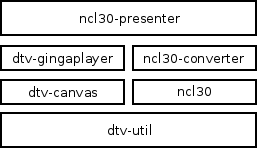
\includegraphics[scale=0.60]{../resources/ginga-modules.png}
\caption{Arquitectura de \emph{Ginga.ar}}
\label{ginga:modules}
\end{figure}
La figura \ref{ginga:modules}, presenta la organización de los mismos.
Los módulos cuyo nombre lleva el prefijo \textit{dtv} fueron desarrollados por el Lifia.\\

\section{Variables de ambiente (Ginga settings)}
Existen un conjunto de variables de ambiente, como por ejemplo \texttt{system.language} (lenguaje del audio) o \texttt{system.subtitle} (lenguaje del subtítulo), que están disponibles para las aplicaciones \texttt{NCLua}, accesibles tanto desde \texttt{NCL} como desde scripts \texttt{Lua}. Las variables se dividen en siete grupos: \texttt{system}, \texttt{user}, \texttt{default}, \texttt{service}, \texttt{si}, \texttt{channel} y \texttt{shared}, cada uno con semántica y características diferentes. Para más información sobre los \texttt{settings} puede consultarse la \texttt{ABNT NBR 15606-2:2007}.

\subsection{Configuración}
Los valores de las variables son configurables por medio de un \texttt{archivo de configuración XML} (ver capítulo \ref{chap:util}) donde cada grupo de variables es un nodo que desciende del nodo \texttt{root}. Las variables de cada grupo son nodos que contienen un valor y descienden del nodo de su grupo.

\begin{lstlisting}[
	language=XML,
	title=Ejemplo de archivo de configuración para las variables de settings,
	keywordstyle=\color{blue},
	commentstyle=\color{gray},
	stringstyle=\color{red},
	tabsize=4,
	showstringspaces=false,
	columns=fullflexible,
	breaklines=true,
	frame=none]
<?xml version="1.0" encoding="UTF-16" standalone="no" ?>
<root>
	<settings>
		<focusBorderTransparencyAsFloat>0</focusBorderTransparencyAsFloat>
	</settings>
	<si>
		<numberOfServices>0</numberOfServices>
		<numberOfPartialServices>0</numberOfPartialServices>
		<channelNumber>0</channelNumber>
	</si>
	<service>
		<currentFocus>0</currentFocus>
		<currentKeyMaster></currentKeyMaster>
	</service>
	<default>
		<focusBorderColor>white</focusBorderColor>
		<selBorderColor>white</selBorderColor>
		<focusBorderWidth>-3</focusBorderWidth>
		<focusBorderTransparency>0</focusBorderTransparency>
	</default>
	<system>
		<audioType>stereo</audioType>
		<audioType0>stereo</audioType0>
		<operatingSystem></operatingSystem>
		<luaVersion>5.1</luaVersion>
		<nclVersion>3.0</nclVersion>
	</system>
</root>
\end{lstlisting}

\subsection{Implementación}
En el archivo \texttt{settings.cpp}, ubicado en la ruta \texttt{lib/dtv-gingaplayer/src/player}, es donde son definidas e inicializadas las variables; cada grupo es representado por un nodo del árbol de configuración, mientras que los valores del mismo son propiedades de dicho nodo; se puede añadir una nueva variable agregando una nueva propiedad al nodo o crear un nodo para conseguir un nuevo grupo de valores. La inicialización de los valores de cada variable puede hacerse al momento de la creación de la propiedad o en la función \texttt{player::settings::load}. Por otro lado, si lo que se desea es modificar un valor ya existente, simplemente bastará con buscar la inicialización de la variable y cambiar su contenido. 
Si sólo se ha modificado un valor de una propiedad o agregado una nueva propiedad a un grupo existente, entonces ésta ya estará disponible para ser usada en las aplicaciones \texttt{NCLua}, sin embargo, agregar un nuevo grupo de variables implica exportarlo a una tabla \texttt{Lua} para poder ser utilizado desde un script, la clase encargada de esto es \texttt{player::settings::Module}, la cual se encuentra en la ruta \texttt{lib/dtv-gingaplayer/src/player/lua/settings}. Durante la inicialización del módulo se llama al método \texttt{exportTables}, en él se hace uso de la clase \texttt{player::settings::UtilCfg2Lua} para exportar la tabla mediante el método \texttt{exportKey}; es aquí donde se debe agregar un llamado extra a éste método para que exporte la clave del nuevo grupo.


\section{Diagramas de secuencia}

\subsection{Inicio de \textit{Ginga.ar}}
En el siguiente diagrama de secuencia se observa el inicio de ejecución de \textit{Ginga.ar}. 
Se instancian los principales objetos de \textit{gingaplayer} como \texttt{System} y \texttt{Device}. 
Luego se inicia la presentación del documento mediante el objeto \texttt{PresentationEngineManager}.

\begin{figure}[ht!]
\centering
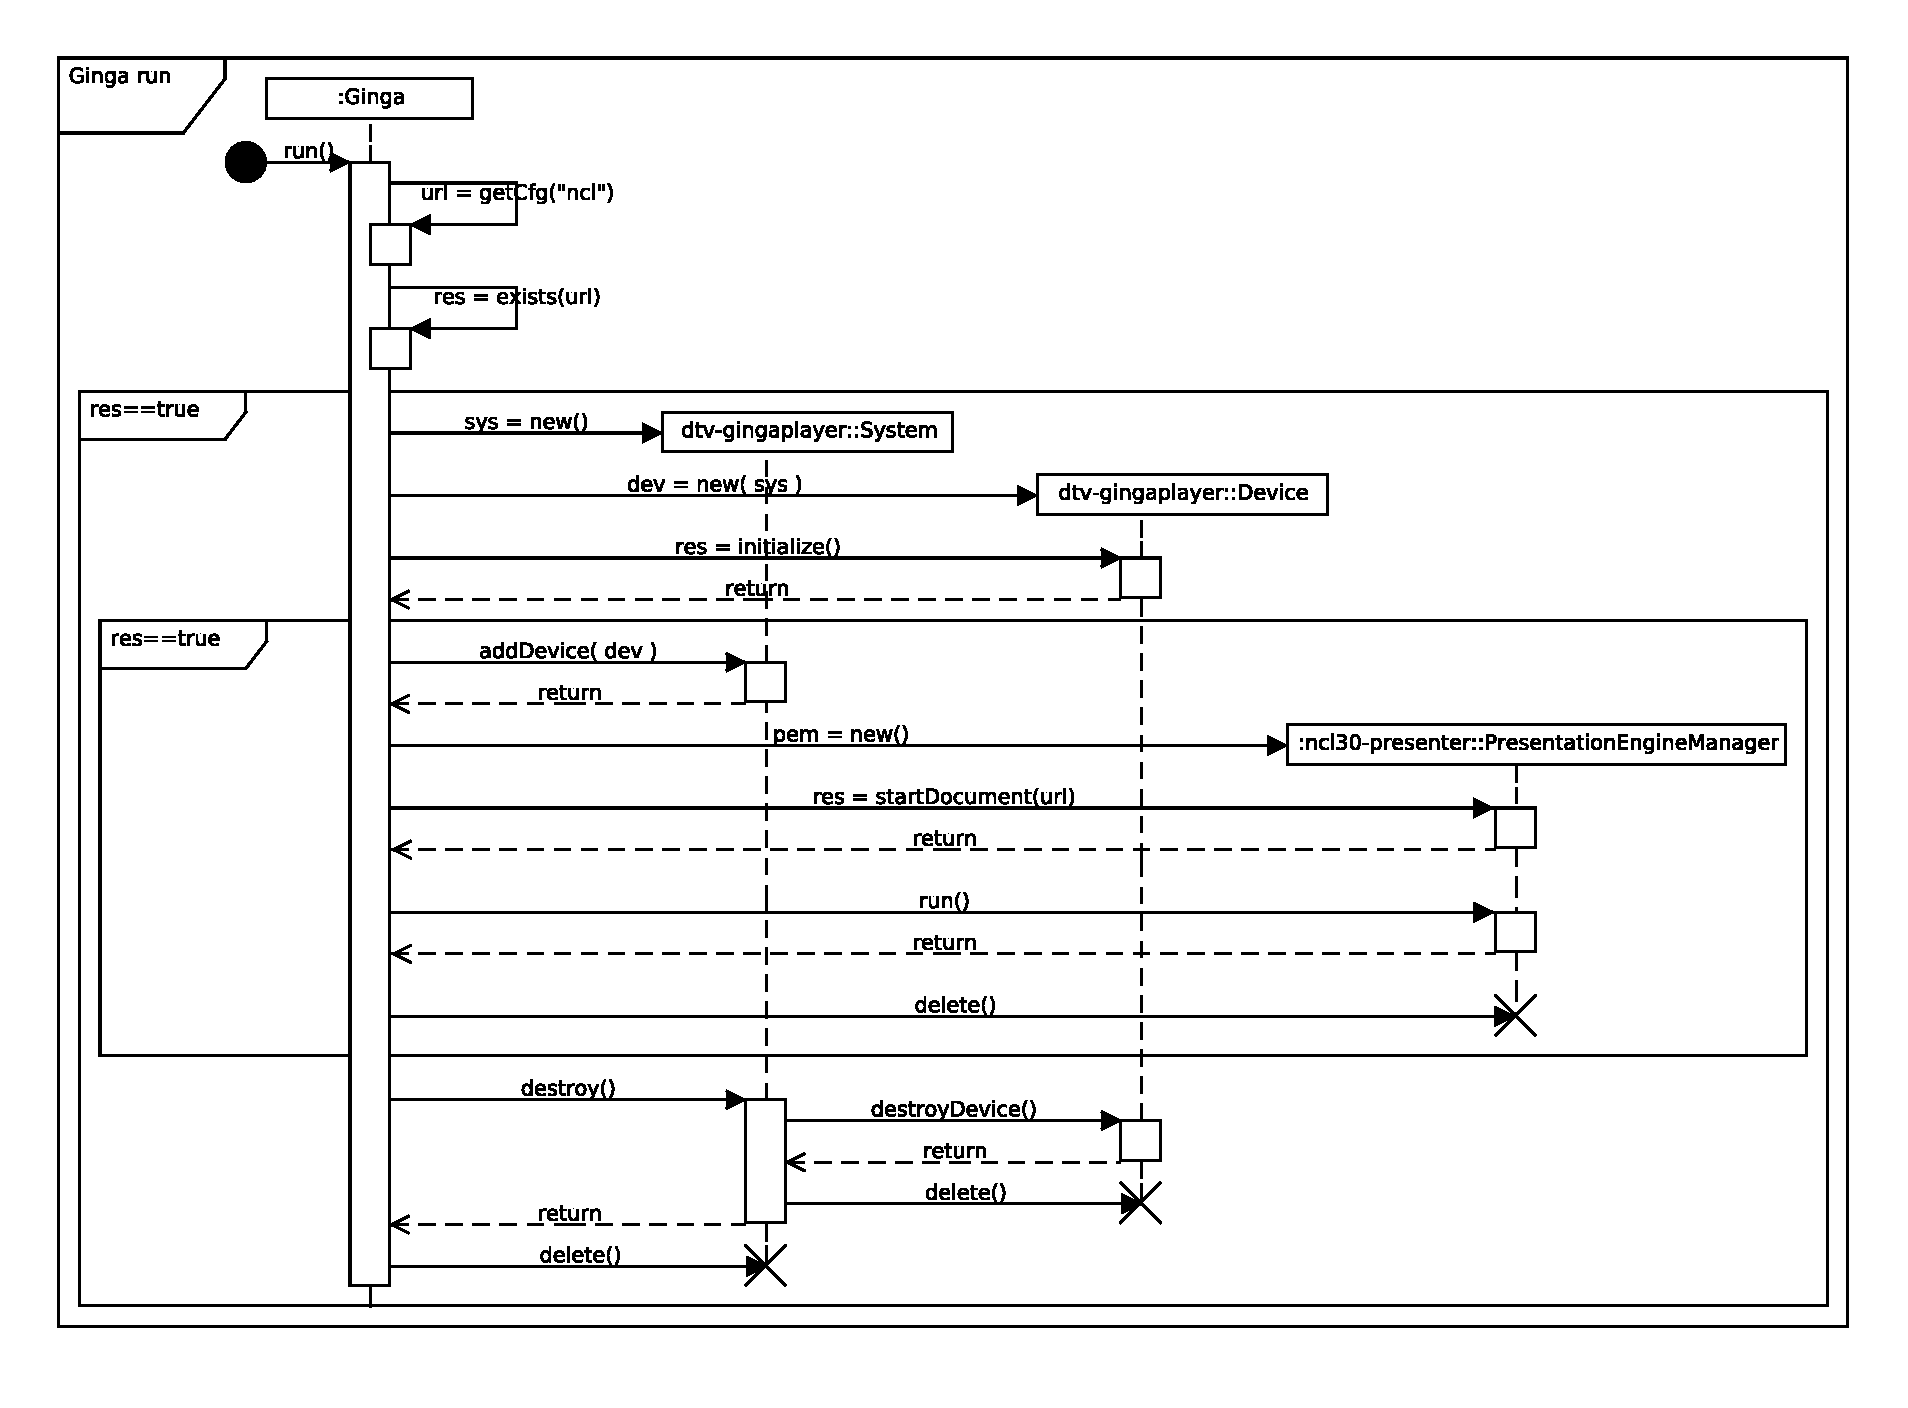
\includegraphics[scale=.5, angle=-90]{../resources/uml-sequence-diagram-ginga-run}
\end{figure}
\clearpage

\subsection{Registro de un \textit{input listener}}
El siguiente diagrama de secuencia muestra como se registra como \textit{input listener} un \texttt{ApplicationPlayerAdapter}.
Este objeto que controla la ejecución de \textit{scripts} \textit{Lua}, es agregado a la colección de \textit{listeners} que 
tiene el objeto \texttt{dtv-gingaplayer::input::Manager}. 

\begin{figure}[ht!]
\centering
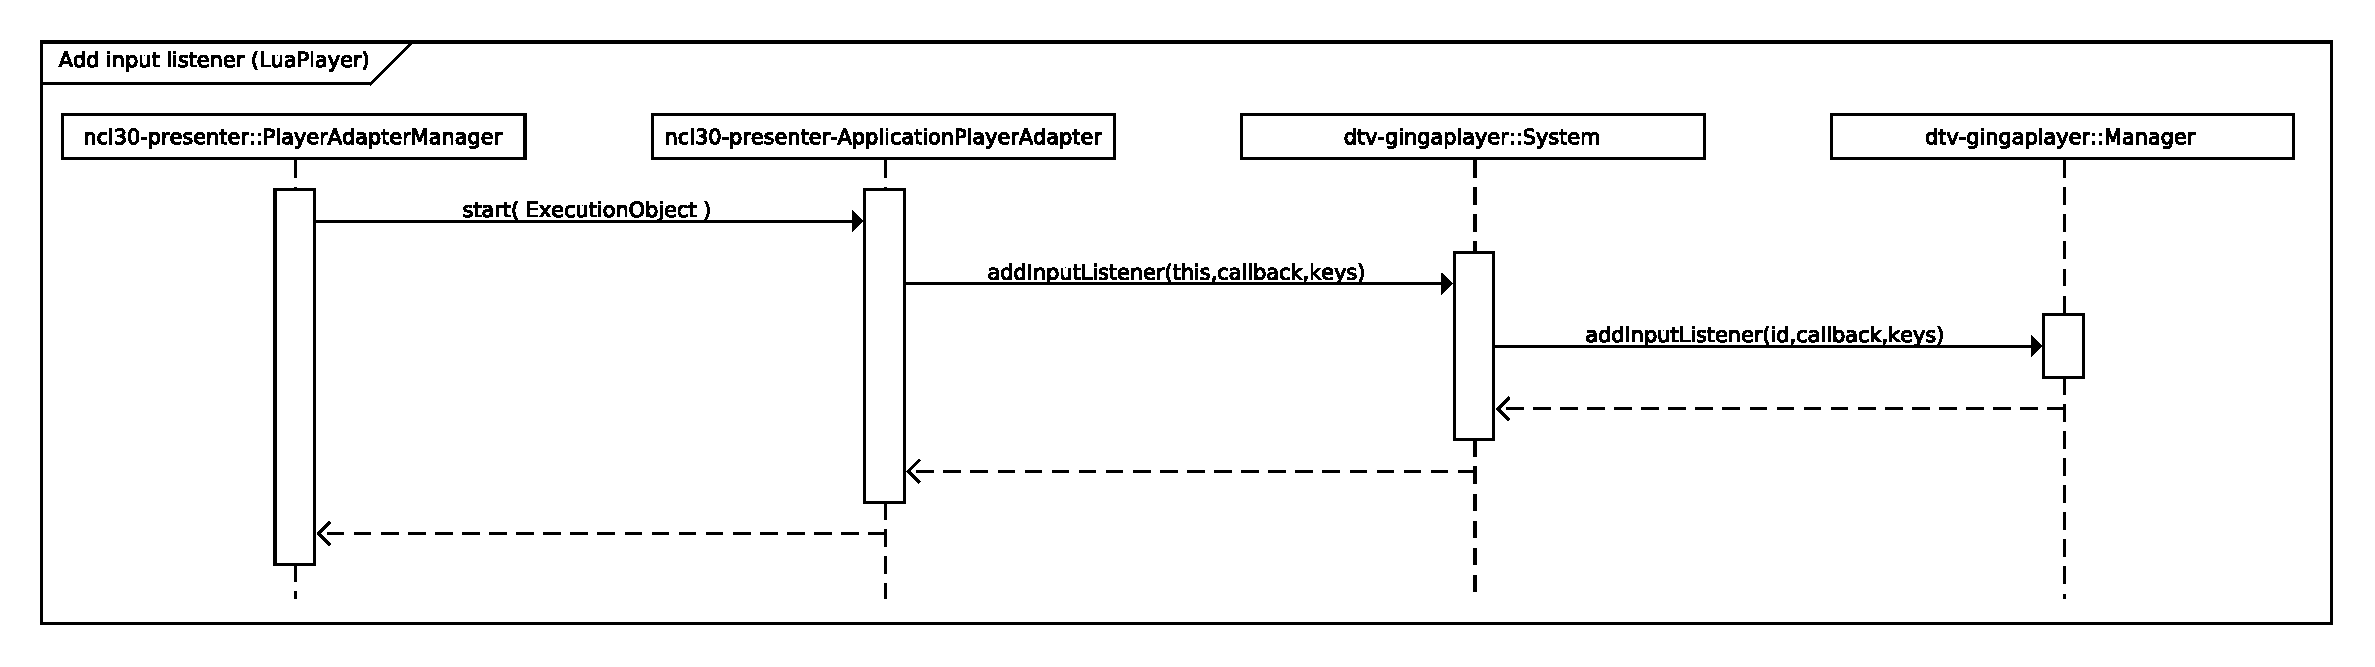
\includegraphics[scale=.4, angle=-90]{../resources/uml-sequence-diagram-keyPress1}
\end{figure}
\clearpage
 
\subsection{\textit{Dispatch} de una tecla}
El siguiente diagrama muestra la interacción que tiene lugar cuando se presiona una tecla en una aplicación.
Se puede ver como la misma es recibida por el \textit{listener} \texttt{ApplicationPlayerAdapter}, registrado en el diagrama anterior.

\begin{figure}[ht!]
\centering
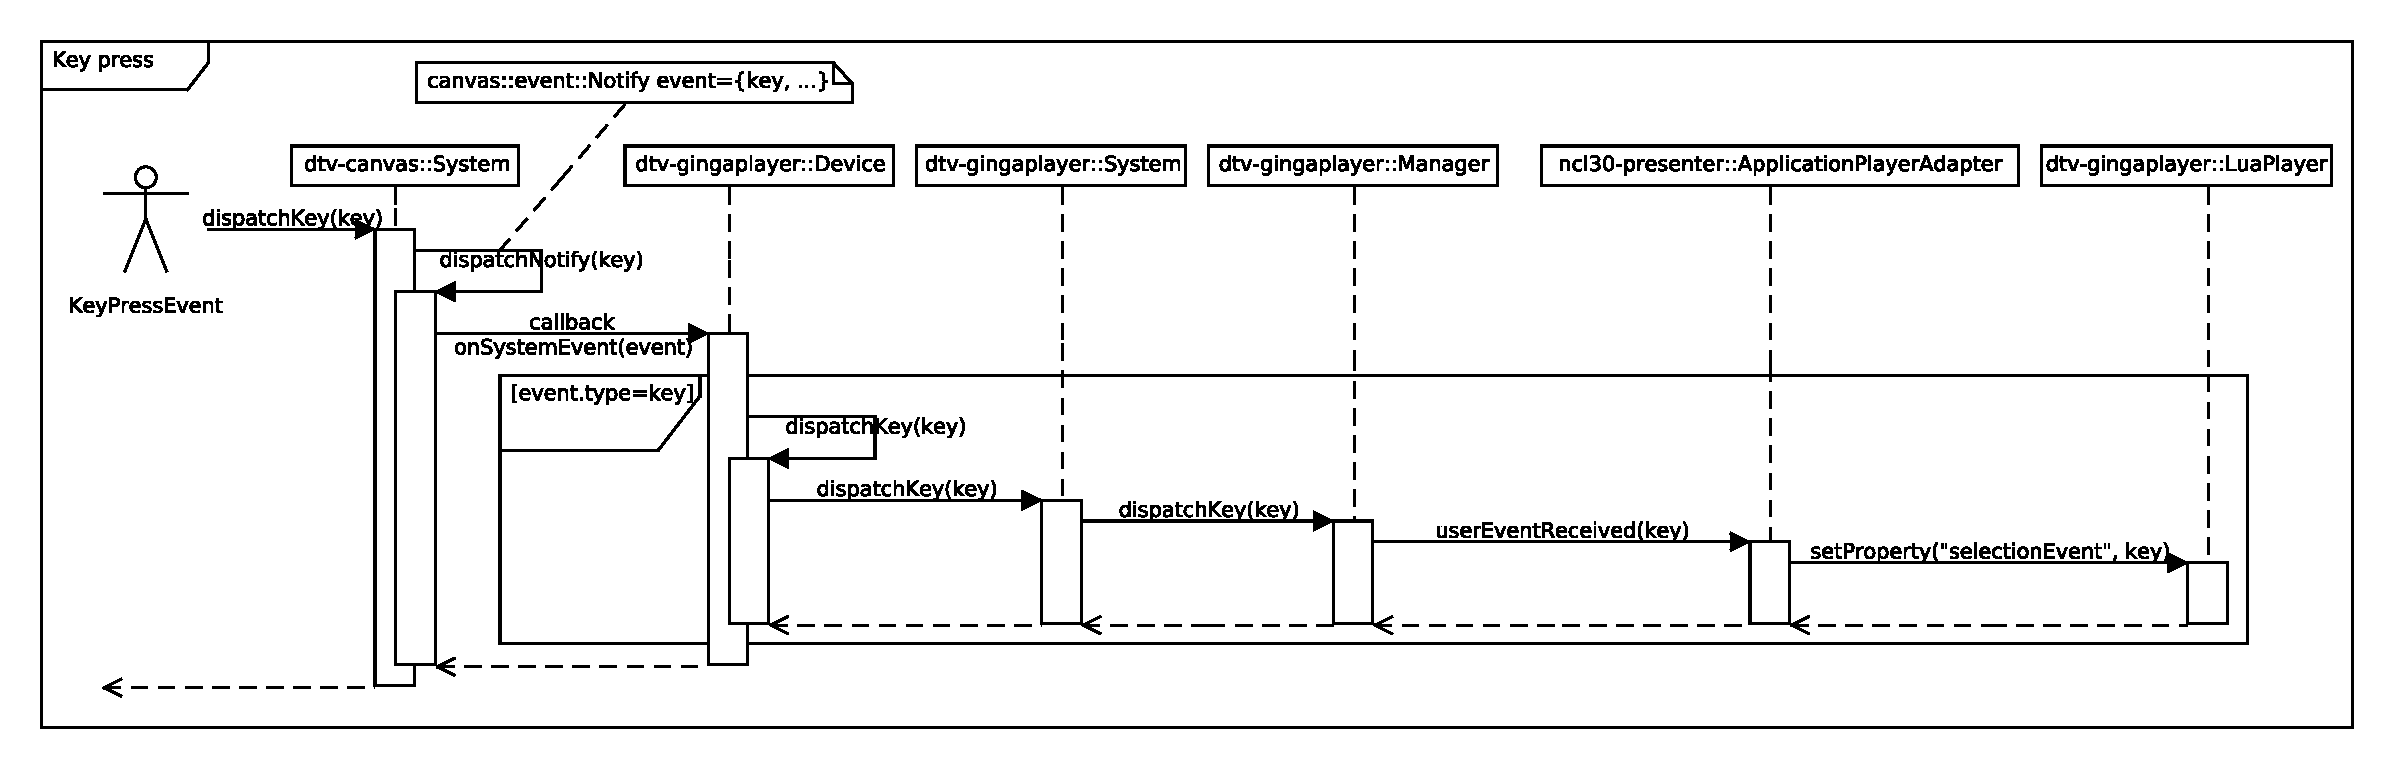
\includegraphics[scale=.4, angle=-90]{../resources/uml-sequence-diagram-keyPress2}
\end{figure}
\clearpage
 
\subsection{Creación de un \textit{player}}
En el siguiente diagrama se muestra como se crea un \textit{player} una vez iniciada la ejecución de \textit{Ginga.ar}. 

\begin{figure}[ht!]
\centering
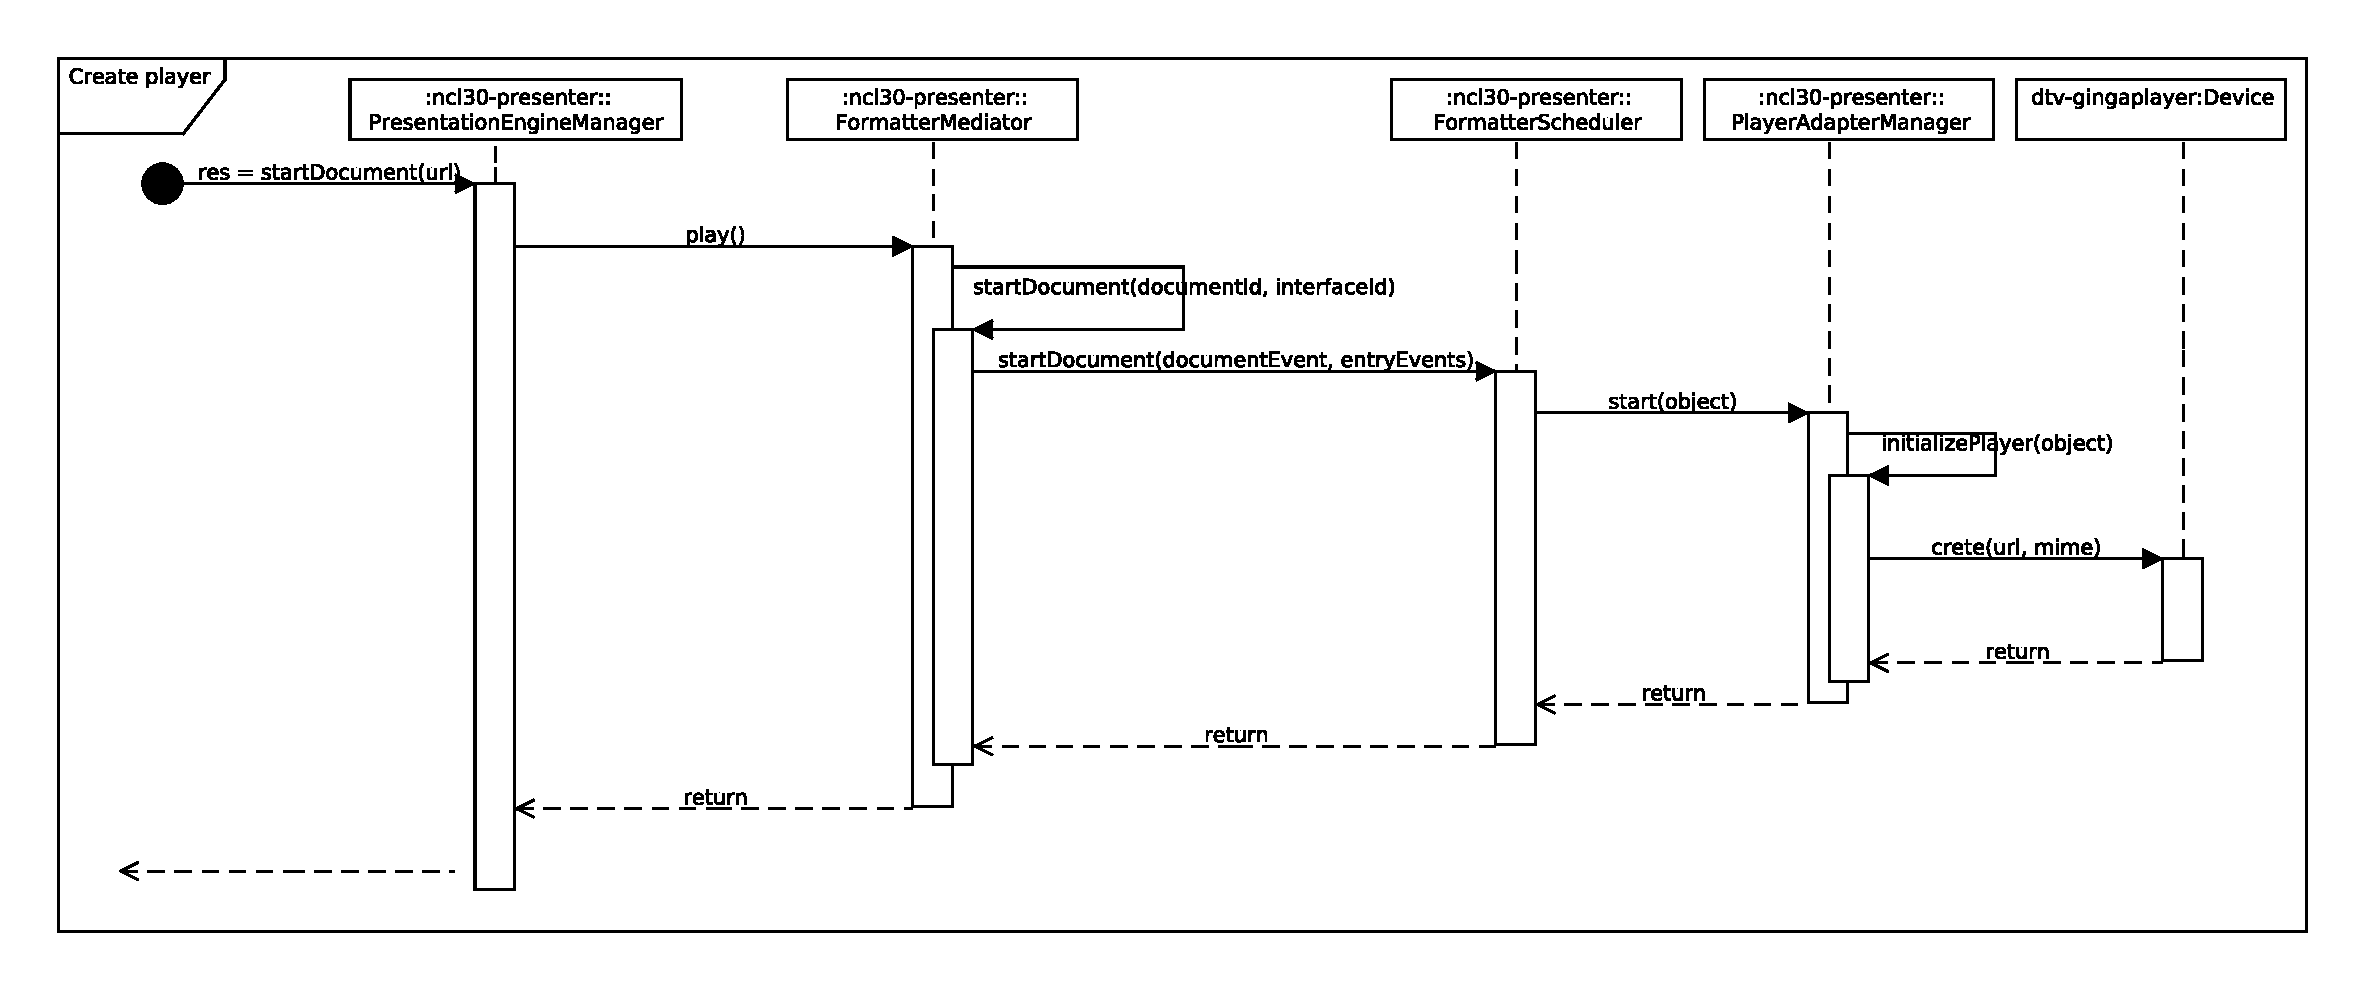
\includegraphics[scale=.4, angle=-90]{../resources/uml-sequence-diagram-playerCreate}
\end{figure}
